% This is "sig-alternate.tex" V2.1 April 2013
% This file should be compiled with V2.5 of "sig-alternate.cls" May 2012
%
% This example file demonstrates the use of the 'sig-alternate.cls'
% V2.5 LaTeX2e document class file. It is for those submitting
% articles to ACM Conference Proceedings WHO DO NOT WISH TO
% STRICTLY ADHERE TO THE SIGS (PUBS-BOARD-ENDORSED) STYLE.
% The 'sig-alternate.cls' file will produce a similar-looking,
% albeit, 'tighter' paper resulting in, invariably, fewer pages.
%
% ----------------------------------------------------------------------------------------------------------------
% This .tex file (and associated .cls V2.5) produces:
%       1) The Permission Statement
%       2) The Conference (location) Info information
%       3) The Copyright Line with ACM data
%       4) NO page numbers
%
% as against the acm_proc_article-sp.cls file which
% DOES NOT produce 1) thru' 3) above.
%
% Using 'sig-alternate.cls' you have control, however, from within
% the source .tex file, over both the CopyrightYear
% (defaulted to 200X) and the ACM Copyright Data
% (defaulted to X-XXXXX-XX-X/XX/XX).
% e.g.
% \CopyrightYear{2007} will cause 2007 to appear in the copyright line.
% \crdata{0-12345-67-8/90/12} will cause 0-12345-67-8/90/12 to appear in the copyright line.
%
% ---------------------------------------------------------------------------------------------------------------
% This .tex source is an example which *does* use
% the .bib file (from which the .bbl file % is produced).
% REMEMBER HOWEVER: After having produced the .bbl file,
% and prior to final submission, you *NEED* to 'insert'
% your .bbl file into your source .tex file so as to provide
% ONE 'self-contained' source file.
%
% ================= IF YOU HAVE QUESTIONS =======================
% Questions regarding the SIGS styles, SIGS policies and
% procedures, Conferences etc. should be sent to
% Adrienne Griscti (griscti@acm.org)
%
% Technical questions _only_ to
% Gerald Murray (murray@hq.acm.org)
% ===============================================================
%
% For tracking purposes - this is V2.0 - May 2012
\documentclass{sig-alternate-05-2015}
\usepackage{hyperref}

% remove copyright space
\makeatletter
\def\@copyrightspace{\relax}
\makeatother

\begin{document}

% --- Author Metadata here ---
%\CopyrightYear{2007} % Allows default copyright year (20XX) to be over-ridden - IF NEED BE.
%\crdata{0-12345-67-8/90/01}  % Allows default copyright data (0-89791-88-6/97/05) to be over-ridden - IF NEED BE.
% --- End of Author Metadata ---

\title{CS388: Assignment-3}
%
% You need the command \numberofauthors to handle the 'placement
% and alignment' of the authors beneath the title.
%
% For aesthetic reasons, we recommend 'three authors at a time'
% i.e. three 'name/affiliation blocks' be placed beneath the title.
%
% NOTE: You are NOT restricted in how many 'rows' of
% "name/affiliations" may appear. We just ask that you restrict
% the number of 'columns' to three.
%
% Because of the available 'opening page real-estate'
% we ask you to refrain from putting more than six authors
% (two rows with three columns) beneath the article title.
% More than six makes the first-page appear very cluttered indeed.
%
% Use the \alignauthor commands to handle the names
% and affiliations for an 'aesthetic maximum' of six authors.
% Add names, affiliations, addresses for
% the seventh etc. author(s) as the argument for the
% \additionalauthors command.
% These 'additional authors' will be output/set for you
% without further effort on your part as the last section in
% the body of your article BEFORE References or any Appendices.

\numberofauthors{1} %  in this sample file, there are a *total*
% of EIGHT authors. SIX appear on the 'first-page' (for formatting
% reasons) and the remaining two appear in the \additionalauthors section.
%
\author{
% You can go ahead and credit any number of authors here,
% e.g. one 'row of three' or two rows (consisting of one row of three
% and a second row of one, two or three).
%
% The command \alignauthor (no curly braces needed) should
% precede each author name, affiliation/snail-mail address and
% e-mail address. Additionally, tag each line of
% affiliation/address with \affaddr, and tag the
% e-mail address with \email.
%
% 1st. author
\alignauthor
Shobhit Chaurasia\\
       \affaddr{Department of Computer Science}\\
       \affaddr{UTEID: sc52987}\\
}
% Just remember to make sure that the TOTAL number of authors
% is the number that will appear on the first page PLUS the
% number that will appear in the \additionalauthors section.

\maketitle

\section{Introduction}
In this assignment, the goal is to incorporate domain adaptation in statistical parsing. A statistical parser trained on a one corpus might learn grammar rules that are specific to the underlying grammatical structure or genre of that corpus. Hence, it makes for an interesting experiment to evaluate the performance of a statistical parser on a different corpus.

One can expect that the parser trained on a ``source'' domain might not perform as well on a "target" domain especially if the two domains are significantly different in terms of genre or style of writing. However, instead of training a parser from scratch for the target domain, we can adapt a parser trained on the source domain to the target domain through \textit{domain adaptation}. In domain adaptation, usually, a small set of labeled examples from the target domain is available to adapt the trained parser to the target domain. In this assignment, we will use a special case of this form of domain adaptation called unsupervised domain adaptation, which represents the worst case scenario - no labeled data from the target domain is made available to the parser.

\section{Unsupervised Domain Adaptation}
In unsupervised domain adaptation, we do not have access to labeled data from the target domain. A parser trained on a source domain is used to produce labels (in this case, parse trees) for sentences from the target domain. This ``self-labeled'' data is then used to re-train the parser along with the gold-labeled data from the source domain. One can repeat the above step multiple times, leading to an approach similar to semi-supervised (hard) EM. In this assignment, though, we re-train the parser using the self-training data only once, and then evaluate its performance on the target domain.

\section{Resources used}
Unlexicalized PCFG \cite{klein2003accurate} from The Stanford Parser package \cite{StanParser} was used to perform the experiments. The two datasets used were the PennTreebank WSJ and Brown datasets.

\section{Experiments}
The experiments involved using a part of WSJ (source domain) as seed set to train the parser, followed by using the trained parser to generate self-training data from unlabeled Brown corpus (target domain), followed by re-training the parser with the original seed set and the self-training data pooled together, and evaluating the parser on the Brown corpus. The experiments also involved switching the roles of the two corpus, and varying the size of the seed set and the self-training set. For comparisons, baseline experiments where the parser is trained and tested on the source domain without self-training, and control experiments where the parser is trained on source domain and tested on target domain without self-training were also performed.

\section{Experiment set-1}
The first set of experiments included using sections 02-22 of WSJ as seed set, followed by using $90\%$ of Brown corpus as self-training set, and performing evaluation on the remaining $10\%$ of Brown corpus. The size of the seed set was varied from $1,000$ to $35,000$ to analyze the effect of increasing seed size on the performance of the parser in the target domain. F1 scores are plotted against the seed set size in Fig.\ref{fig:1-seed}. 

As evident from the red curve, the F1 score increases with increase in the size of seed set. This is expected, since a larger seed set trains a better parser initially, which enables better parses (i.e. fewer incorrect parses) to be generated for the self-training set, thereby increasing the quality of pseudo-supervision for the final training.

A Control experiment (green curve in Fig. \ref{fig:1-seed}) was also performed in which the parser was trained using WSJ as the seed set, and evaluated on the Brown corpus (the same $10\%$ as before) without performing self-training. The curve shows a similar increasing pattern as the learning curve for the previous setting because a larger seed set trains a better parser. However, the performance without self-training is always worse than the performance with self-training (by $1-4.7$ points), thereby indicating that domain adaptation even in a completely unsupervised manner is useful. This should not be surprising, because the parser trained using the seed set does indeed generate a ``decent'' self-training set which has at least a small fraction of correctly parsed sentences. The pooling of the original seed set and this ``decent'' self-training induces some amount of target domain knowledge into the training set, thereby training a better parser overall (for the target domain). Further, the difference in the F1 score between the parser with and without self-training gradually decreases (from $\approx4.7$ points to $\approx1$ point) as the size of seed set is increased. This is because once the seed size is sufficiently large, the \emph{difference} in the quality of pseudo-supervision due to addition of more seed examples fades out since this addition, while being useful, does not alter the parser's learned hypothesis significantly.

Further, an in-domain (Baseline) experiment (blue curve in Fig. \ref{fig:1-seed}) was performed to evaluate the performance of the parser which was trained on WSJ, on WSJ itself, without self-training. Once again, the performance increases with increase in the size of the seed set for the reasons mentioned above. Moreover, as expected, the in-domain F1 score is significantly better than the out-of-domain F1 score (by $4-7$ points), because the parser is primarily trained on WSJ corpus, and has better learned the underlying structure of WSJ as compared to that of a new domain. The self-training in the first case is merely pseudo-supervision, and not enough to adapt the parser as well to Brown as it is to WSJ on which it was originally trained (with real-supervision).

Something that's worth noting is that the rate of increase in F1 score in all the three settings decreases with increase in the size of seed set. This is because initially, when the size of the seed set is fairly small (e.g., less than $10,000$), the addition of more seed examples helps train a better parser. This is because a small seed set does not provide enough data to the parser to learn different nuances of the corpus, and addition of new seed examples provides significant amount of valuable supervision . However, when the parser is already trained on a sufficiently large seed set (e.g., greater than $20,000$), it has probably already learned quite a lot about the corpus (provided the seed set was reflective of the universe), and additional seed examples, while being useful, do not provide significantly newer information to the parser.

\begin{figure}
\centering
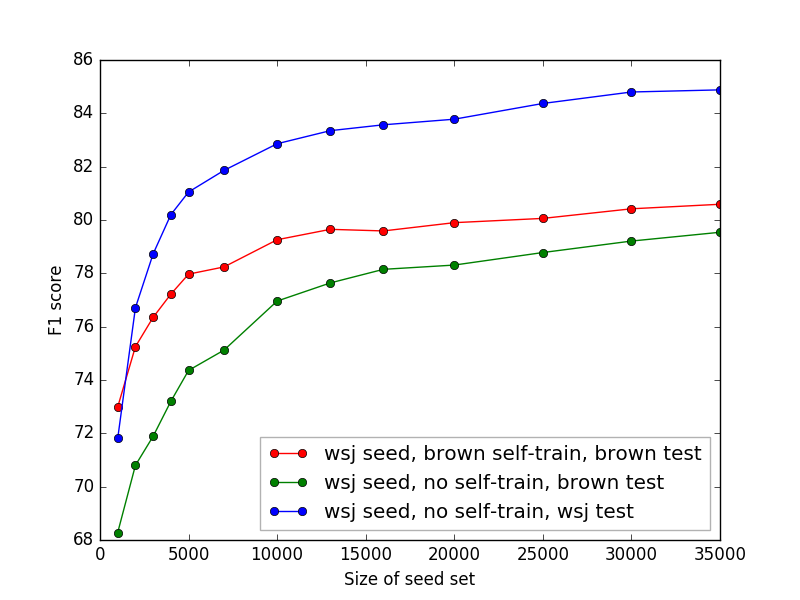
\includegraphics[width=0.95\columnwidth]{figs/fig-1-seed}
\caption{F1 score as a function of the size of seed set. The green curve corresponds to the Control setting. The blue curve corresponds to the Baseline setting.}
\label{fig:1-seed}
\end{figure}

\section{Experiment-2}
This is similar to the first experiment in that sections 02-22 of WSJ were used as seed set to train a parser, followed by using $90\%$ of Brown corpus for self-training, and evaluation was done on the remaining $10\%$ of Brown corpus. However, instead of varying the size of seed set, the aim of this experiment was to analyze the effect of the size of self-training set on the parser's performance. The size of seed set was fixed at 10,000 parse trees from WSJ, while the size of self-training set was varied from $1000$ to $21,000$. The F1 scores are plotted against the self-training set size in Fig.\ref{fig:2-self}.

There is a general increasing trend in the F1 score as the size of self-training set is increased which is because a larger self-training set provides the parser with more supervision to learn from. However, one must not forget that this supervision could be highly noisy, which is potentially why there is a meager drop in F1 score ($79.13$ to $79.08$) on increasing the size of self-training set from $13,000$ to $17,000$, and a less than usual increase at $4000$.

It should be noted that the magnitude of increase in F1 score as the size of self-training set is increased from $1000$ to $21,000$ (keeping seed set fixed) is only $\approx1.5$ points (see Fig. \ref{fig:2-self}) as compared to $~7$ points increase when the size of seed set is increased from $1000$ to $20,000$ (keeping self-training set fixed; see Fig. \ref{fig:1-seed}). Although this comparison is not totally fair, it reflects how valuable seed-supervision (in the form of gold-labeled examples) is over the noisy pseudo-supervision (in the form of self-trained examples). Nonetheless, gold-labeled data is hard to collect, while self-training is free of cost, and the fact that it can boost the performance even by a small amount is amazing.

\begin{figure}
\centering
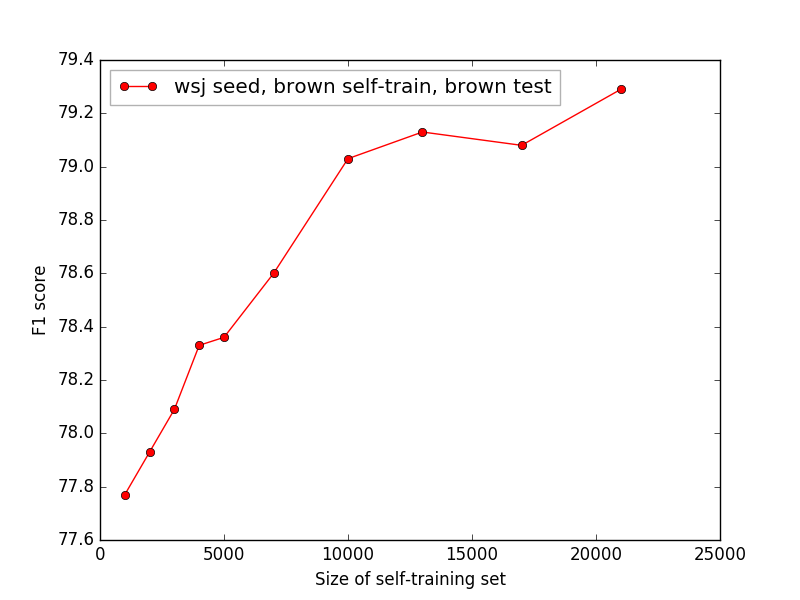
\includegraphics[width=0.95\columnwidth]{figs/fig-2-self}
\caption{F1 score as a function of size of self-training set, with $10,000$ seed examples.}
\label{fig:2-self}
\end{figure}

\section{Experiment set-3}
The intent behind these set of experiments is, in essence, same as that behind the Experiment set-1. However, the source and target domains were flipped. This set of experiments included using $90\%$ of the Brown corpus as the seed set, followed by using sections $02-22$ of WSJ as self-training set, and evaluating on section 23 of WSJ corpus. The size of the seed set was varied from $1,000$ to $21,000$ to analyze the effect of increasing seed size on the performance of the parser in target domain. The F1 scores are plotted against the seed set size in Fig.\ref{fig:3-seed}. 

The general trends are similar to those in experiment set-1, and hence, the corresponding observations will only be briefly stated here without full explanations to avoid repetition. An important observation is that the F1 scores in all the three settings in this set of experiments (with Brown as source domain and WSJ as target domain) are in general lower than their counter-parts in experiment set-1 (with WSJ as source domain, and Brown as target domain). This is because the Brown corpus has a wider spectrum of genres than WSJ, and hence is harder to learn.

As evident from the red curve, the F1 score increases with increase in the size of seed set. This is expected, since a larger seed set trains a better parser.

A Control experiment (green curve in Fig. \ref{fig:3-seed}) was also performed in which the parser was trained using Brown as the seed set, and evaluated on the WSJ corpus (section $23$) without performing self-training. The curve shows a similar increasing pattern as the learning curve for the previous setting because a larger seed set trains a better parser. However, the performance without self-training is always worse than the performance with self-training (by $3.5-7.5$ points), thereby indicating that domain adaptation even in a completely unsupervised manner is useful. The difference is more pronounced here than the difference when WSJ was the source domain, indicating that self-training is more useful when Brown is the source and WSJ is the target domain, as compared to the setting with WSJ as source and Brown as target domain because of WSJ's ``specificity'' and Brown's generic nature.

The reason why unsupervised domain-adaptation works better for going from Brown to WSJ than the other way round is two-fold:
\begin{enumerate}
\item Brown is a more generic corpus with multiple genres, while WSJ is a highly specific one - it contains only news-wire articles. Domain adaptation from a generic corpus to a highly specific corpus is easier than the other way round.
\item The self-training data generated out of the Brown corpus by a parser trained on WSJ is expected to be of poorer quality than the one generated out of WSJ by a parser trained on Brown. This is because the parser trained on WSJ will have poorer generalization (in terms of performance on other genres) than the one trained on Brown.
\end{enumerate}


Further, an in-domain experiment (blue curve in Fig. \ref{fig:3-seed}) was performed to evaluate the performance of the parser which was trained on Brown, on Brown itself, without self-training. Once again, the performance increases with increase in the size of the seed set. Here also, the in-domain F1 score is significantly better than the out-of-domain F1 score (by $8-10$ points)

\begin{figure}
\centering
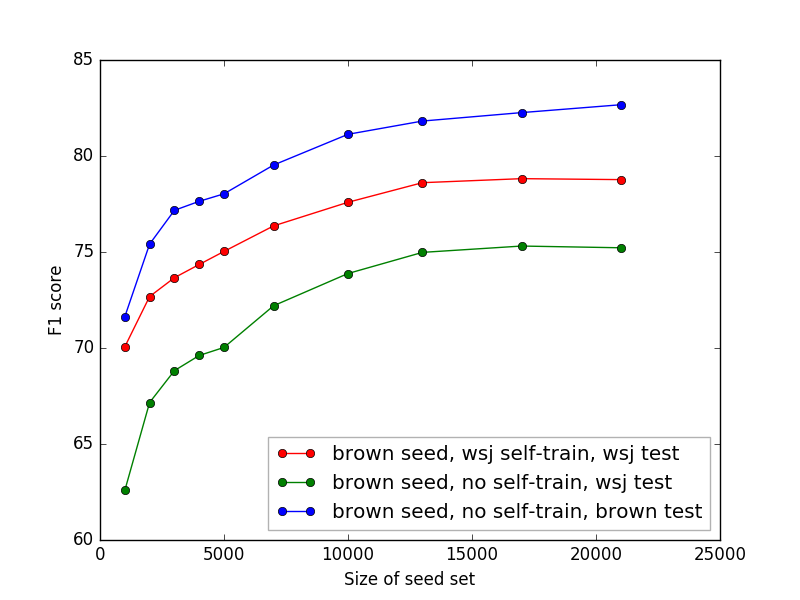
\includegraphics[width=0.95\columnwidth]{figs/fig-3-seed}
\caption{F1 score as a function of size of seed set. The green curve corresponds to the Control setting. The blue curve corresponds to the in-domain setting.}
\label{fig:3-seed}
\end{figure}

\section{Experiment-4}
This is, in essence, similar to experiment-2, with source and target domains flipped - $90\%$ of the Brown corpus was used as the seed set, followed by sections $02-22$ of WSJ used as self-training set, and evaluation done on section 23 of WSJ corpus. The aim of this experiment was to analyze the effect of the size of self-training set on the parser's performance. The size of seed set was fixed at 10,000 parse trees from Brown, while the size of self-training set was varied from $1000$ to $35,000$. The F1 scores are plotted against the self-training set size in Fig.\ref{fig:4-self}.

Once again, the general observations are similar to that in experiment-2, and hence, will only be briefly stated here. As pointed out in the previous section, F1 scores in this setting (with Brown as seed and WSJ as self-training/testing) are in general lower than their counter-parts in experiment-2 (with WSJ as seed, and Brown as self-training/testing).

There is a general increasing trend in the F1 score as the size of self-training set is increased which is because a larger self-training set provides the parser with more supervision to learn from. However, one must not forget that this supervision could be highly noisy, which is potentially why there are meager drops in F1 scores in a couple of places on increasing the size of self-training set.

\begin{figure}
\centering
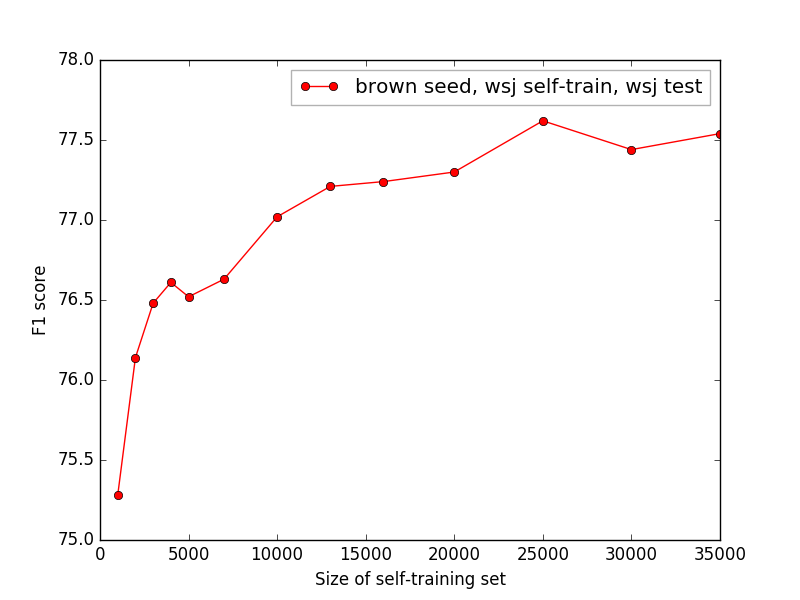
\includegraphics[width=0.95\columnwidth]{figs/fig-4-self}
\caption{F1 score as a function of size of self-training set, with $10,000$ seed examples.}
\label{fig:4-self}
\end{figure}

\section{Comparison with paper}
The observations drawn from the above experiments are in line with the results obtained in \cite{reichart2007self}. This is despite the fact that the parser used in \cite{reichart2007self} is the Collins parser, which is different from the one used in these experiments. This further affirms the conclusion that self-training is indeed useful for domain adaptation, and that this is not necessarily an artifact of the strength or weakness of a specific parser.

\section{Conclusion}
The results strongly suggest that self-training is a powerful method for domain adaptation. Its impact is especially profound when the seed training set is small. Even in settings with larger seed sets, an increase of even a couple of points of F1 score for free that it provides (without the need for additional labeled data from target domain) is impressive. We also learned that not only is the size of seed set important, but also that the size of the self-training set can make a huge difference.

\bibliographystyle{acm}
\bibliography{bib}
\end{document}
